\section{Aerodynamic concept analysis}
\label{ch:aero_analysis}
In order to analyse the aerodynamic characteristics of the proposed concepts a software tool was developed. This chapter will deal with the development and implementation of this program. The aerodynamic tool is 
developed to be able to assess the performance of the different system concepts on the different trade-off criteria as defined in Chapter \label{ch:trade-offcriteria}: the lift gradient \gls{sym:cla-alpha} relates to the deceleration time and the moment stability \gls{sym:cma-alpha} relates to the static stability of the decelerator. In order to calculate these values, the concept shapes are discretised in triangles, and for each triangle the pressure coefficient \gls{sym:cp} is calculated. This can then be integrated over the surface to obtain lift, drag and moment. Also, the maximum heat flux \gls{sym:qw} is determined for each concept, which is used to determine the thermal protection system mass. First section \ref{subsec:aerotool} will discuss the tool development process. Secondly section \ref{subsec:appaeroanal} 

\subsection{Development of aerodynamic analysis tool}
\label{subsec:aerotool}
For analysing the aerodynamic characteristics of each concept the modified Newtonian method will be used. This method relates the inclination angle $\gls{sym:chi}$ of a flat plate with respect to an incoming flow to the magnitude of its coefficient of pressure, as shown in equation \ref{eq:modnewtonian} \cite{AndersonJr.2006}.
\begin{multicols}{2}
\begin{equation}
\gls{sym:CP}=\gls{sym:CP}_{max}sin^{2}(\gls{sym:chi})
\label{eq:modnewtonian}
\end{equation} \break
\begin{equation}
\gls{sym:CP}_{max}=\frac{p_{O_{2}}-p_{\infty}}{\frac{1}{2}\rho_{\infty}V_{\infty}^{2}}
\label{eq:cpmax}
\end{equation}
\end{multicols}
In equation \ref{eq:modnewtonian} $\gls{sym:CP}_{max}$ is the value of $\gls{sym:CP}$ in the stagnation point of an arbitrary body. Since the stagnation point is per definition located behind a normal shock its value can be found from the normal shock relations. The result of doing this is shown in equation \ref{eq:cpmax}. Here $p_{O_{2}}$ denotes the total pressure in the stagnation point and can be found using equation \ref{eq:po2} \cite{AndersonJr.2007}.

\begin{equation}
\frac{p_{O_{2}}}{p_{\infty}}=\left(\frac{(\gls{sym:gamma}+1)^{2}M_{\infty}^{2}}{4\gls{sym:gamma} M_{\infty}^{2}-2(\gls{sym:gamma}-1)}\right)^{\frac{\gls{sym:gamma}}{\gls{sym:gamma}-1}}\left(\frac{1-\gls{sym:gamma}+2\gls{sym:gamma} M_{\infty}^{2}}{\gls{sym:gamma}+1}\right)
\label{eq:po2}
\end{equation}

Furthermore it can be noted that $\frac{1}{2}\rho_{\infty}V_{\infty}^{2}=\frac{\gls{sym:gamma}}{2}p_{\infty}M_{\infty}^{2}$ \cite{AndersonJr.2007}. Combining this with equation \ref{eq:cpmax} produces equation \ref{eq:cpmaxfinal}, where the ratio $\frac{p_{O_{2}}}{p_{\infty}}$ can be calculated using equation \ref{eq:po2}.

\begin{equation}
C_{p_{max}}=\frac{2}{\gls{sym:gamma} M_{\infty}^{2}}\left(\frac{p_{O_{2}}}{p_{\infty}}-1\right)
\label{eq:cpmaxfinal}
\end{equation}

By dividing the surface of the body to be analysed into many triangular elements the pressure coefficient distribution of said body can be determined numerically. A velocity magnitude is given as input, together with the angle of attack \gls{sym:alpha} and sideslip angle \gls{sym:beta}. Following this the outward surface normal vector is computed in Cartesian coordinates for every element, after which the velocity unit vector is computed with equation \ref{eq:unitV}. To determine $sin(\gls{sym:chi})$ for every element the dot product of the velocity unit vector with the surface normal vector is then taken, as shown in equation \ref{eq:dotproduct}.
\begin{multicols}{2}
\begin{equation}
\gls{sym:Vhat}=\frac{\gls{sym:Vv}}{\gls{sym:V}}
\label{eq:unitV}
\end{equation} \break
\begin{equation}
sin(\gls{sym:chi})=\gls{sym:Vhat} \bullet \gls{sym:n}
\label{eq:dotproduct}
\end{equation}
\end{multicols}
Using $C_{p_{max}}$ and $sin(\gls{sym:chi})$ the \gls{sym:CP} for every surface element is calculated, after which it is multiplied with the element area and the element surface normal vector. This results in an elemental pressure force in three dimensions from which the lift and drag forces can be determined. By then summing the resultant forces for all elements the total body forces are found. Next to the body forces the resultant aerodynamic moment can also be found. For this the location of the \acrfull{cg} is used as input, after which the moments about the \gls{cg} caused by the force on each element can be summed. 


Two notes are made here with regard to the results produced by the Newtonian flow method:
\begin{itemize}
	\item The accuracy of the Newtonian and modified Newtonian methods increases as \gls{sym:M} become higher \cite{AndersonJr.2007,Bertin1994}
	\item Newtonian and modified Newtonian theory is more accurate for three-dimensional bodies than it is for two-dimensional cases \cite{AndersonJr.2007}
\end{itemize}

In addition to determining the aerodynamic forces and moments acting on the body, the heat flux in the stagnation point is also computed. A generalized Equation to predict the heat flux on a body can be found in \cite{AndersonJr.2006,Tauber1986}. This  is shown in Equation \ref{eq:heatflux}.

\begin{equation}
\gls{sym:qw}=\rho_{\infty}^{N}V_{\infty}^{M}C
\label{eq:heatflux}
\end{equation}

In the stagnation point it is furthermore known that: 
\begin{multicols}{2}
\begin{equation}
\label{eq:stagdens}
N=0.5
\end{equation} \break
\begin{equation}
\label{eq:stagspeed}
M=3.0
\end{equation}
\end{multicols}
\begin{equation}
\label{eq:stagcoefficient}
C=1.83 \times 10^{-8} R^{-\frac{1}{2}}\left(1-\frac{h_{w}}{h_{0}}\right)
\end{equation}
Where in Equation \ref{eq:stagcoefficient} $R$ denotes the local body radius in the stagnation point and $h_{w}$ and $h_{0}$ comprise of the wall and total enthalpies respectively. An additional assumption that is made here is that $\frac{h_{w}}{h_{0}}\ll 1$. Justification for this statement can be found in the fact that the wall temperature must be smaller than the melting or decomposition temperature during the entire flight. Thus, although the temperature can become very high, the resulting wall enthalpy $h_{w}$ will still be much smaller than the total enthalpy $h_{0}$ \cite[p.347]{AndersonJr.2006}. %In addition to this the computed heat flux will increase as a result of neglecting this factor. One can see that if in later design phases the enthalpy ratio is included into the calculations this will relax the design constraints.
Combining Equations \ref{eq:heatflux}, \ref{eq:stagdens}, \ref{eq:stagspeed}, \ref{eq:stagcoefficient} into one single equation produces:
\begin{equation}
\gls{sym:qw}_{stagnation}=1.83 \times 10^{-8}\rho_{\infty}^{0.5} V_{\infty}^{3.0} R^{-\frac{1}{2}}
\label{eq:qstag}
\end{equation}
Where $\gls{sym:qw}_{stagnation}$ denotes the heat flux into the body at the stagnation point. This will be used as input for the thermodynamic model in order to compute the required thicknesses of the \acrfull{tps} lay-up.

\subsection{Model verification \& validation}
\label{subsec:aeroverval}
After the model construction verification was carried out to determine whether the model correctly implemented the calculations of the modified Newtonian method. This was done by placing two triangular surface elements in a flow. First at an angle and secondly normal to the flow. The model outputs were verified by also calculating the results by hand.

Following the verification process the model was validated using experimental values of different parameters. Each separate validation case will be treated here.

\subsubsection{\gls{sym:CD}-validation against experimental drag of a sphere}
\label{subsubsec:valsphere}
For the first model validation case a comparison was made the between the \gls{sym:CD}-value of a sphere in hypersonic flow that were computed by the model and as found in an experiment. It was found that for hypersonic Mach numbers the experimental \gls{sym:CD}-value of a sphere is $0.92$ \cite{Bailey1966,AndersonJr.2007,Cox1965}. When computing \gls{sym:CD} numerically with the modified Newtonian method using $>10,000$ surface elements produces $\gls{sym:CD}=0.916$, which coincides with a discrepancy of $0.5\%$ of the experimental value. Since the accuracy of the experimental data is approximately $\pm1.5\%$ \cite{Bailey1966} this discrepancy falls within the confidence interval of the measurements.

\subsubsection{\gls{sym:CP}-validation against experimental data of a sharp cone}
\label{subsubsec:valsharpconeCP}
Following the \gls{sym:CD}-validation for blunt bodies presented in the previous section now \gls{sym:CP}-validation will be carried out for sharp bodies. This is carried out by comparing the \glspl{sym:CP} at several points on the surface of a cone with half-cone angle \gls{sym:theta} of $15$ degrees. The experimental data was collected for $\gls{sym:M}=14.9$ and $\gls{sym:gamma}=\frac{5}{3}$ (helium was used as medium) \cite{Bertin1994,Cleary1970}. Figure \ref{fig:CPcone30val} shows the data points that were collected for angles of attack $\gls{sym:alpha}=10\deg$ and $\gls{sym:alpha}=20\deg$ in figure \ref{fig:CPconealpha10} and \ref{fig:CPconealpha20} respectively. On the X-axis the variable \gls{sym:beta_cone} is used. This quantity refers to the local cross-sectional surface rotation with respect to an axis that is defined positive in the positive Z-direction. Figure \ref{fig:beta_cone} showcases this concept more clearly. Normally the domain of \gls{sym:beta_cone} lies between $0\deg$ and $360\deg$, but because the cone is symmetrical only half of the cone surface is plotted here. Furthermore, since the cone in question is a sharp cone with a constant semi-cone angle the \gls{sym:CP}-distribution is constant along the cone surface for constant \gls{sym:beta_cone}.
As can be seen in figures \ref{fig:CPconealpha10} and \ref{fig:CPconealpha20} the modified Newtonian method is the most accurate around $\gls{sym:beta_cone}=90\deg$.

\begin{figure}[h]
	\centering
	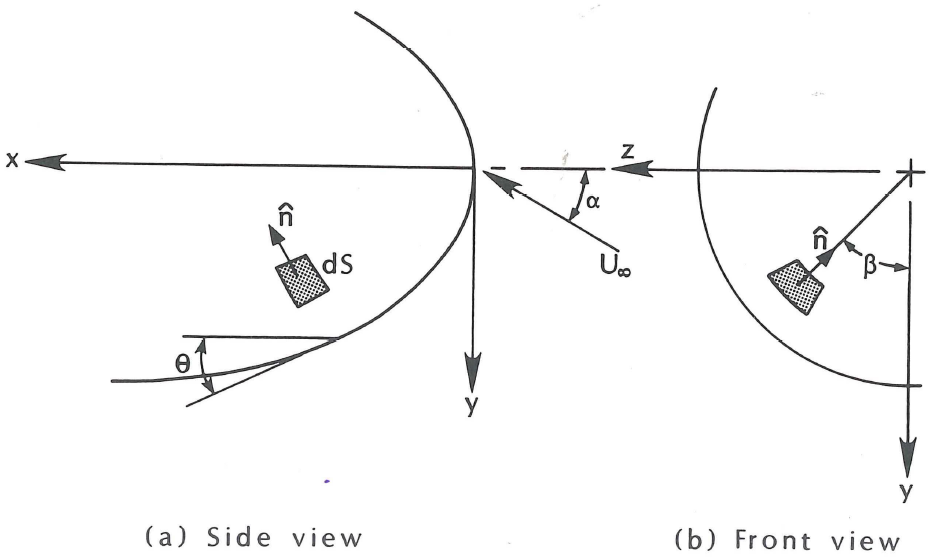
\includegraphics[width=0.7\textwidth]{./Figure/def_beta}
	\caption{Definition of \gls{sym:beta_cone} \cite{Bertin1994}}
	\label{fig:beta_cone}
\end{figure}

\begin{figure}[h]
	\centering
	\begin{subfigure}[b]{0.49\textwidth}
		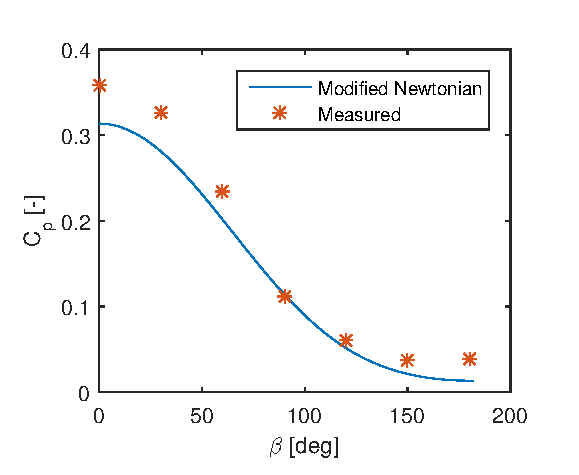
\includegraphics[width=0.96\textwidth]{./Figure/cone30deg_alpha10}
		\caption{$\gls{sym:alpha}=10\deg$}
		\label{fig:CPconealpha10}
	\end{subfigure}
		\begin{subfigure}[b]{0.49\textwidth}
			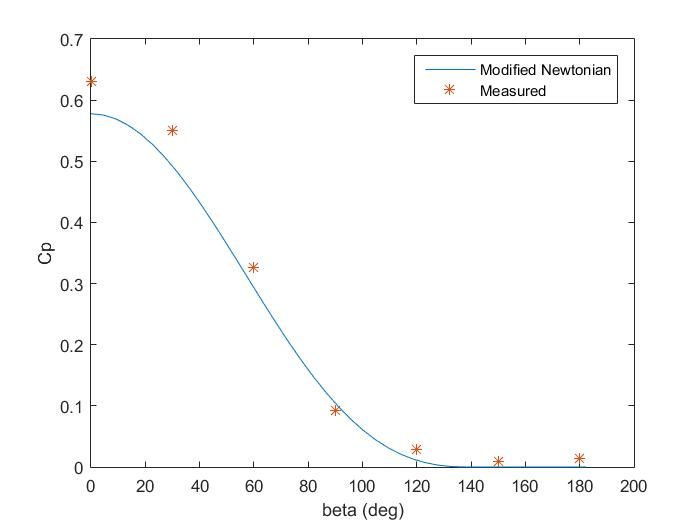
\includegraphics[width=0.96\textwidth]{./Figure/cone30deg_alpha20}
		\caption{$\gls{sym:alpha}=20\deg$}
		\label{fig:CPconealpha20}
	\end{subfigure}
	\caption{Comparisons between experimental and numerical \glspl{sym:CP}}
	\label{fig:CPcone30val}
\end{figure}

\subsubsection{\gls{sym:CD}-validation against experimental data of a sharp cone}
\label{subsubsec:valsharpconeCD}
Stevens found that for a sharp cone-cylinder with a half-cone angle \gls{sym:theta} of $30\deg$ $\gls{sym:CD}=0.58$ in an air-stream of Mach $8$ where angle of attack \gls{sym:alpha} and sideslip angle \gls{sym:beta} are zero \cite{Stevens1950,AndersonJr.2007}. The numerical model predicts for this case that $\gls{sym:CD}=0.456$, which coincides with a discrepancy of $21.4\%$ of the experimental value. This is in line with the results of figure \ref{fig:CPcone30val} where the \glspl{sym:CP} predicted by the numerical model were smaller than the experimental values of a sharp cone.

\subsubsection{\gls{sym:CP}-validation against experimental data of the Apollo re-entry capsule}
\label{subsubsec:Apollo_validation}
The data points in figure \ref{fig:Apollo_cp} represent pressure coefficients measured at various locations of one of the two axisymmetric axes \cite{Bertin1966}. The quantity shown on the X-axis is defined in figure \ref{fig:Apollo_y}. As can be seen in figure \ref{fig:Apollo_cp} the numerical model is most accurate around the centre of the capsule. As the distance to the centreline increases, so does the discrepancy between the experimental and numerical values.

\begin{figure}[H]
	\centering
	% This file was created by matlab2tikz.
% Minimal pgfplots version: 1.3
%
\definecolor{mycolor1}{rgb}{0.20810,0.16630,0.52920}%
\definecolor{mycolor2}{rgb}{0.19855,0.72140,0.63095}%
%
\begin{tikzpicture}

\begin{axis}[%
width=0.95092\figurewidth,
height=\figureheight,
at={(0\figurewidth,0\figureheight)},
scale only axis,
unbounded coords=jump,
xmin=-1.5,
xmax=1.5,
xlabel={$\frac{s}{R}$ [-]},
xmajorgrids,
ymin=0,
ymax=1.8,
ylabel={$C_p$ [-]},
ymajorgrids,
legend style={at={(0.5,0.03)},anchor=south,legend cell align=left,align=left,draw=white!15!black}
]
\addplot [color=mycolor1,solid]
  table[row sep=crcr]{%
-1.095	0.00194223338446491\\
-1.09496992147514	0\\
-1.09472939221993	0.0105764109659139\\
-1.09463923908848	0\\
-1.09415883985204	0.0286612804702033\\
-1.09400885921748	0\\
-1.09328990674072	0.0560242775566994\\
-1.09308050968954	0\\
-1.09212497457122	0.092367937353207\\
-1.09185673504618	0\\
-1.09066723634165	0.137297047773714\\
-1.09034088956864	0\\
-1.08892068761116	0.190322850013229\\
-1.08853712808401	0\\
-1.08689011554844	0.250868241388263\\
-1.08645039457714	nan\\
-1.08458108581034	0.318273930108563\\
-1.0819999272869	0.3918054818373\\
-1.07915371475421	0.470661188513422\\
-1.07605024948299	0.55398068095838\\
-1.07269803785581	0.640854198362098\\
-1.06910626805175	0.730332419944821\\
-1.06528478486218	0.821436757031353\\
-1.06124406270688	0.913169997566455\\
-1.05699517692443	1.00452718986455\\
-1.05254977341541	1.09450664823589\\
-1.04792003672184	1.18212096017887\\
-1.0431186566302	1.26640787317747\\
-1.03815879338958	1.34644093888065\\
-1.03305404164036	1.42133979364298\\
-1.02781839315226	1.42835417521564\\
-1.01832656548985	1.44935521736688\\
-0.986104624404206	1.50751538767456\\
-0.953709183690762	1.52351962805163\\
-0.921145943147255	1.5390688207566\\
-0.888420632094868	1.55415195599687\\
-0.855539008370191	1.56875835245074\\
-0.822506857312158	1.58287766497233\\
-0.789329990744154	1.59649989205813\\
-0.75601424595145	1.60961538306931\\
-0.72256548465417	1.62221484520418\\
-0.688989591975953	1.63428935021542\\
-0.655292475408497	1.64583034086682\\
-0.621480063772172	1.6568296371244\\
-0.587558306172872	1.66727944207735\\
-0.553533170955306	1.67717234758383\\
-0.519410644652901	1.68650133963741\\
-0.485196730934503	1.69525980344988\\
-0.450897449548067	1.7034415282464\\
-0.416518835261513	1.71104071176934\\
-0.382066936800948	1.71805196448708\\
-0.347547815786417	1.72447031350459\\
-0.312967545665402	1.7302912061727\\
-0.27833221064423	1.73551051339311\\
-0.243647904617593	1.74012453261658\\
-0.208920730096357	1.74412999053202\\
-0.174156797133862	1.74752404544416\\
-0.139362222250891	1.7503042893381\\
-0.104543127359504	1.75246874962895\\
-0.0697056386859186	1.75401589059533\\
-0.0348558856926369	1.75488268492153\\
-0	1.75525426236477\\
0.0348558856926369	1.75488268492153\\
0.0697056386859186	1.75401589059533\\
0.104543127359504	1.75246874962895\\
0.139362222250891	1.7503042893381\\
0.174156797133862	1.74752404544416\\
0.208920730096357	1.74412999053202\\
0.243647904617593	1.74012453261658\\
0.27833221064423	1.73551051339311\\
0.312967545665402	1.7302912061727\\
0.347547815786417	1.72447031350459\\
0.382066936800948	1.71805196448708\\
0.416518835261513	1.71104071176934\\
0.450897449548067	1.7034415282464\\
0.485196730934503	1.69525980344988\\
0.519410644652901	1.68650133963741\\
0.553533170955306	1.67717234758383\\
0.587558306172872	1.66727944207735\\
0.621480063772172	1.6568296371244\\
0.655292475408497	1.64583034086682\\
0.688989591975953	1.63428935021542\\
0.72256548465417	1.62221484520418\\
0.75601424595145	1.60961538306931\\
0.789329990744154	1.59649989205813\\
0.822506857312158	1.58287766497233\\
0.855539008370191	1.56875835245074\\
0.888420632094868	1.55415195599687\\
0.921145943147255	1.5390688207566\\
0.953709183690762	1.52351962805163\\
0.986104624404206	1.50751538767456\\
1.01832656548985	1.44935521736688\\
1.02781839315226	1.42835417521564\\
1.03305404164036	1.42133979364298\\
1.03815879338958	1.34644093888065\\
1.0431186566302	1.26640787317747\\
1.04792003672184	1.18212096017886\\
1.05254977341541	1.09450664823589\\
1.05699517692443	1.00452718986455\\
1.06124406270688	0.913169997566455\\
1.06528478486218	0.821436757031353\\
1.06910626805175	0.730332419944821\\
1.07269803785581	0.640854198362098\\
1.07605024948299	0.55398068095838\\
1.07915371475421	0.470661188513422\\
1.0819999272869	0.3918054818373\\
1.08458108581034	0.318273930108563\\
1.08645039457714	nan\\
1.08689011554844	0.250868241388263\\
1.08853712808401	0\\
1.08892068761116	0.190322850013229\\
1.09034088956864	0\\
1.09066723634165	0.137297047773714\\
1.09185673504618	0\\
1.09212497457122	0.0923679373532069\\
1.09308050968954	0\\
1.09328990674072	0.0560242775566994\\
1.09400885921748	0\\
1.09415883985204	0.0286612804702033\\
1.09463923908848	0\\
1.09472939221993	0.0105764109659139\\
1.09496992147514	0\\
1.095	0.0019422333844649\\
};
\addlegendentry{Modified Newtonian};

\addplot [color=mycolor2,only marks,mark=asterisk,mark options={solid}]
  table[row sep=crcr]{%
-1.02718093698553	0.326751322056051\\
-0.951551131339198	1.02168543257076\\
-0.799264139197169	1.4880212545932\\
-0.247616441864002	1.7300201625693\\
0.0180691662280614	1.74873159897289\\
0.273850147488554	1.70299372722051\\
0.547682381293604	1.63105638244619\\
0.68183629061674	1.49350323432687\\
0.817930550476365	1.44043342939967\\
0.871460439771112	1.37207156639853\\
0.929404854806911	1.26182928317321\\
0.981710021888355	0.939565894363321\\
1.0408671541418	0.31807000221393\\
1.09530512997895	0.0391870122023066\\
};
\addlegendentry{Measured};

\end{axis}
\end{tikzpicture}%
	\caption{Comparison between experimental and numerical \gls{sym:CP}'s for the Apollo re-entry capsule}
	\label{fig:Apollo_cp}
\end{figure}

\begin{figure}[H]
	\centering
	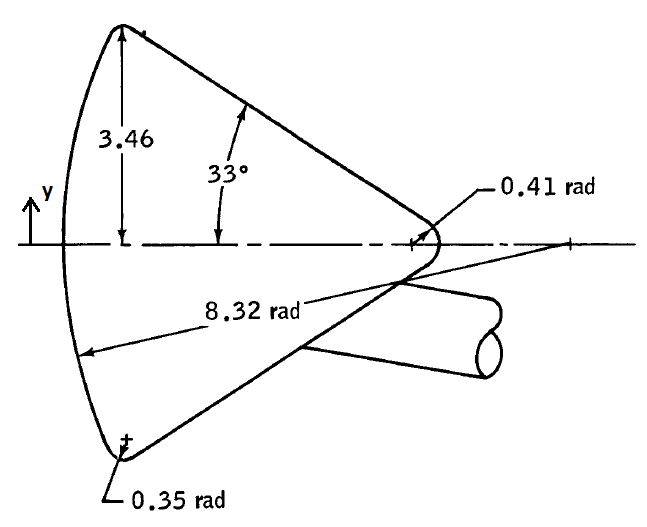
\includegraphics[width=0.4\textwidth]{./Figure/Apollo_model}
	\caption{Definition of unit on the X-axis of figure \ref{fig:Apollo_cp} \cite{Bertin1966}}
	\label{fig:Apollo_y}
\end{figure}

\subsubsection{Maximum heat flux validation against experimental data of the \gls{irve} 3 vehicle}
\label{subsubsec:heatvalidation}
Dillman et al. observed that the maximum heat flux on the \acrfull{irve} 3 was $14.4$ $\frac{W}{cm^{2}}$ during re-entry at an altitude of $50$ kilometres and Mach $7.0$ \cite{Dillman2012}. The maximum heat flux computed by the numerical tool in the stagnation point for these flow conditions is $11.7$ $\frac{W}{cm^{2}}$. This is equal to $81.0\%$ of the experimental value. Thus a discrepancy of $19.0\%$ is present between the experimental and numerical maximum heat fluxes.

\subsection{Conclusions after the validation procedure}
\label{subsec:validconclusions}

From section \ref{subsec:aeroverval} it can be concluded that the accuracy of the modified Newtonian method varies between geometries. The \gls{sym:CD} predicted in section \ref{subsubsec:valsphere} is accurate to within $1\%$ of the experimental value, whereas the accuracy of the \gls{sym:CP} in section \ref{subsubsec:valsharpconeCP} varied over the cone surface. This discrepancy was also observed in section \ref{subsubsec:valsharpconeCD}, where the difference between the numerical and experimental \gls{sym:CD} was $21.4\%$, and again for the Apollo capsule in section \ref{subsubsec:Apollo_validation}. After judging the accuracy shown in figures \ref{fig:CPcone30val} and \ref{fig:Apollo_cp} it was determined that the accuracy of the modified Newtonian method is adequate for the conceptual and preliminary design phases.


The model for the maximum heat flux found on a body was validated in section \ref{subsubsec:heatvalidation}. It was observed that a discrepancy of $19.0\%$ was present between the numerical and experimental maximum heat fluxes. After consideration this was deemed to be acceptable for conceptual and preliminary design.

\subsection{Application of analysis tool to system concepts}
\label{subsec:appaeroanal}
After the model development and validation, the different system concepts are evaluated for their performance in the different trade-off criteria. Specifically, the lift, moment and aerodynamic heating are discussed. They are all related to the trade-off criteria as defined in Chapter \ref{ch:tradeoff}. Firstly, the relation between the aerodynamic properties and the trade-off criteria is discussed. After that, the results from the aerodynamic analysis are given.

\subsubsection{Trade-off criteria justification} \label{sec:tradeoffaero}
In this section, the quantification method of the trade-off criteria relating to aerodynamics is justified.

The stability trade-off criterion is given by the static stability of the vehicle. This is characterised by the pitch moment gradient \gls{sym:cma-alpha}: For a negative \gls{sym:cma-alpha}, a positive angle of attack leads to a negative moment, such that the angle of attack is restored by the induced moment. This leads to a spacecraft that is less reactant to disturbances in the atmosphere, which leads to a less strict requirement on the control system to keep the spacecraft pointed in the desired direction. A positive value of \gls{sym:cma-alpha} means the spacecraft is not stable, and the control system will have to very actively monitor the spacecraft in order for it to not diverge from the required attitude. \\


Aerodynamic drag is used as the method to decelerate the vehicle from the initial velocity to $\gls{sym:M}=5$ before landing. The drag equation is given in Eq. \ref{eq:drag}.

\begin{equation} \label{eq:drag}
\gls{sym:D} = \frac{1}{2}\gls{sym:rho}\gls{sym:V}^2\gls{sym:cda}
\end{equation}
\begin{equation} \label{eq:lift}
\gls{sym:L} = \frac{1}{2}\gls{sym:rho}\gls{sym:V}^2\gls{sym:cla}
\end{equation}

The lift is defined as the component of the aerodynamic force perpendicular to the flow, where the direction away from Mars is defined positive. The drag component is defined parallel to the flow. For blunt bodies in hypersonic flow with the blunt side pointed towards the oncoming flow, a positive angle of attack results in a negative lift.

The drag and lift are dependent on the drag and lift coefficients of the spacecraft as well as the density. As can be seen in Figure \ref{fig:atmos_height_rho}, the density is significantly higher in lower parts of the atmosphere. For a given \gls{sym:cda}, the maximum deceleration can be chosen by varying the lowest part of the orbit: a higher density compensates for a low drag coefficient to produce the same force as a spacecraft with a high drag coefficient and a low density. Because of the large variation of density in the atmosphere, it is possible to find a trajectory for any \gls{sym:cda}. Thus, the drag coefficient itself is not a key driver for the design. However, the spacecraft can influence its deceleration time in the atmosphere by producing lift: if the spacecraft were to fly out of the atmosphere, a downward pointing lift would divert it's trajectory more through the atmosphere. The ability of the spacecraft to influence this trajectory through the atmosphere is characterised by the amount of lift that can be produced, with respect to the amount of drag produced at the same \gls{sym:alpha}. The dependence on drag is due to the fact that two spacecraft with the same \gls{sym:clcd} but a different \gls{sym:cda}, will just have the lowest part of the trajectory in a different height, where the total lift and drag force will be the same for both spacecraft. Therefore, the deceleration time is characterised by \gls{sym:clcd}. \\

The mass of the decelerator is composed of the structural mass, the \gls{tps} mass and the control system mass.

The \gls{tps} mass is estimated based on the heat load on the spacecraft, which is the integral of the heat flux over time. This heat load is the total amount of heat supplied to the spacecraft between initial entry and final descent, and estimates the total amount of energy the \gls{tps} has to withstand. This can thus be used to size the thickness of the \gls{tps}, which leads directly to the mass of the system.

The control system mass is based on the moment that the control system has to provide. The amount of lift that a spacecraft has to produce in order to attain a desirable orbit directly dictates the angle of attack. This angle of attack, in turn, determines the moment that the control system has to compensate in order to maintain the required angle of attack. It is thus not the moment coefficient itself that has to be minimised, but rather the amount of moment that is needed to provide a certain amount of lift. Therefore, the ratio \gls{sym:cmcl} is used to quantify the control system mass. \\


\begin{figure}[h]
	\centering
	\begin{subfigure}[b]{0.49\textwidth}
		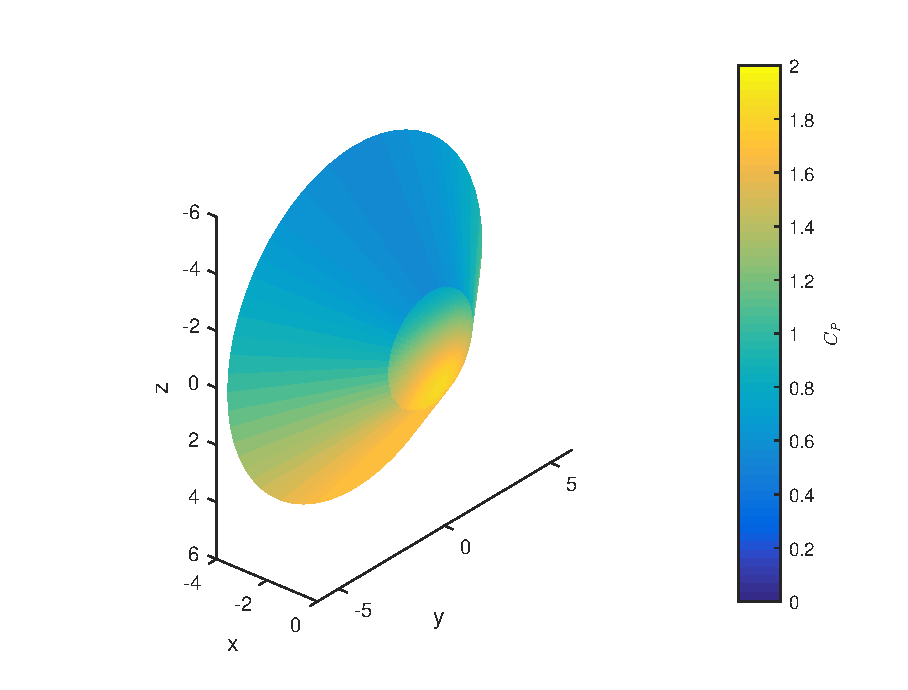
\includegraphics[width=0.96\textwidth]{./Figure/aero_model/irve.eps}
		\caption{Stacked toroid, tension cone}
		\label{fig:cpstackedtoroid}
	\end{subfigure}
	\begin{subfigure}[b]{0.49\textwidth}
		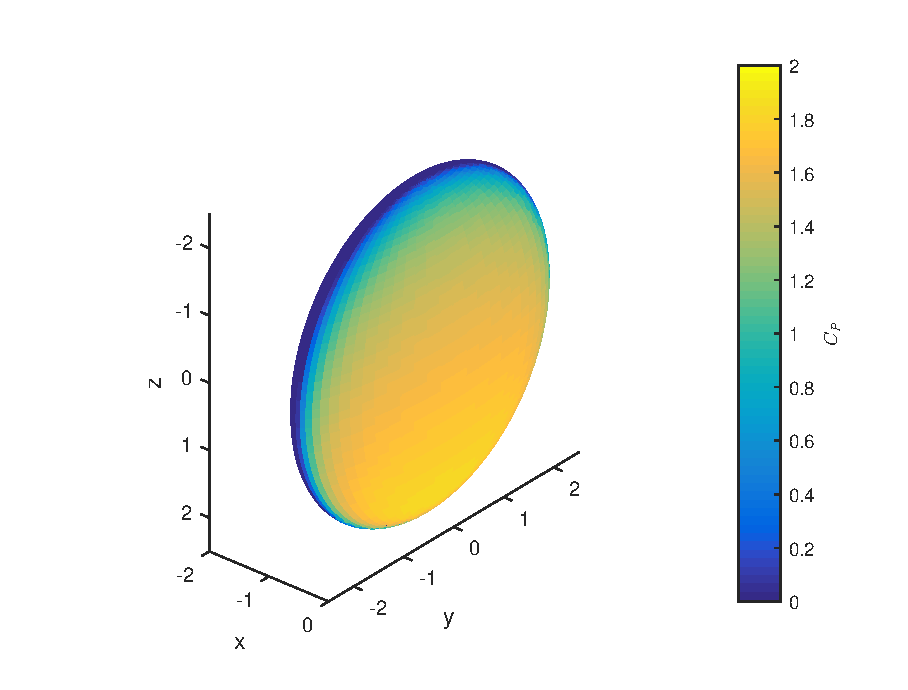
\includegraphics[width=0.96\textwidth]{./Figure/aero_model/rigid.eps}
		\caption{Rigid structure}
		\label{fig:cprigid}
	\end{subfigure}
	\begin{subfigure}[b]{0.49\textwidth}
		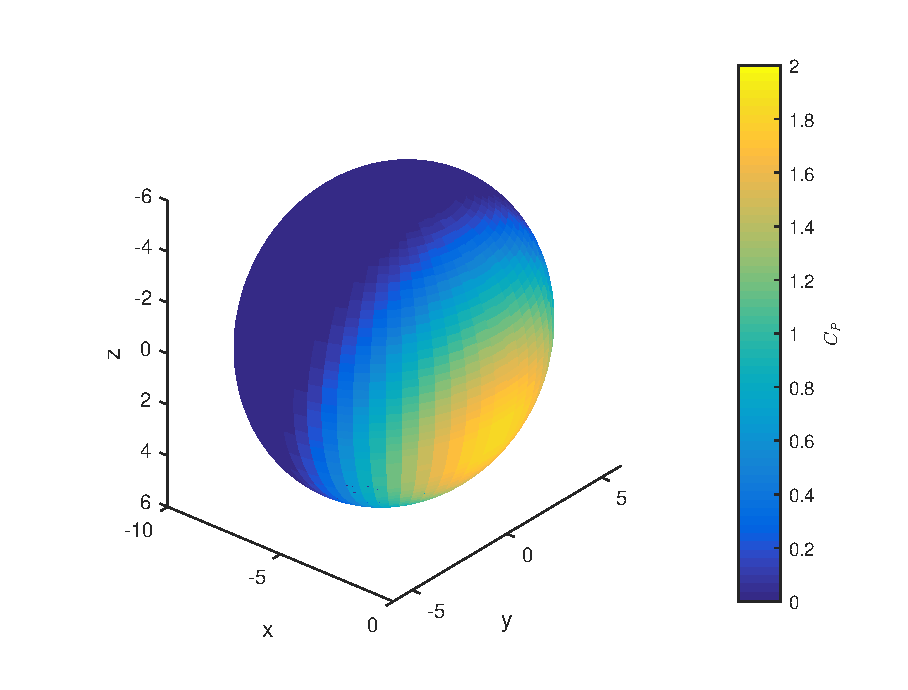
\includegraphics[width=0.96\textwidth]{./Figure/aero_model/isotensoid.eps}
		\caption{Isotensoid}
		\label{fig:cpisotensoid}
	\end{subfigure}
	\begin{subfigure}[b]{0.49\textwidth}
		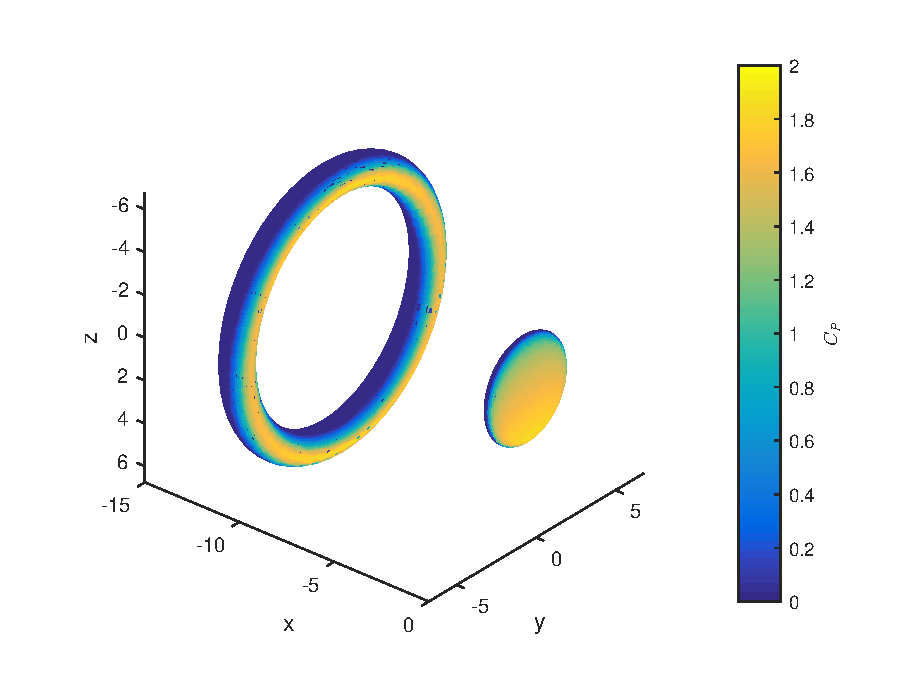
\includegraphics[width=0.96\textwidth]{./Figure/aero_model/ballute.eps}
		\caption{Trailing ballute}
		\label{fig:cpballute}
	\end{subfigure}	
	\caption{Geometry and pressure coefficient \gls{sym:CP} distribution over the different concepts, at an angle of attack $\gls{sym:alpha}=20[deg]$. $\gls{sym:M}=23.3$, $\gls{sym:gamma}=1.4$}
	\label{fig:conceptscp}
\end{figure}



In order to assess these values, a representative geometry is chosen. Since Newtonian flow only affects the parts of the vehicle that are in direct line of sight of the oncoming flow, only the front of the decelerator has to be accurately modelled. The stacked toroid and tension cone concepts are modelled after the \gls{irve} missions as flown by NASA, as can be seen in Figure \ref{fig:cpstackedtoroid}. The rigid concept's front is a largely flattened sphere, as seen in Figure \ref{fig:cprigid}. The isotensoid is modelled as a slightly flattened sphere, with a radius of 6 meters perpendicular and a radius of 5 meter in direction of the flow. This model can be seen in Figure \ref{fig:cpisotensoid}. The trailing ballute is modelled as a single torus trailing a body comparable to the rigid concept, as seen in Figure \ref{fig:cpballute}, and 



\subsubsection{Deceleration performance}
$\gls{sym:clcd}$ is the lift coefficient divided by the drag coefficient. In Figure \ref{fig:clcd}, a graph is presented showing the lift over drag ratios of the different concepts for different angles of attack.

\begin{figure}[b]
	\setlength\figureheight{0.8\textwidth} 
	\setlength\figurewidth{0.75\textwidth}
	% This file was created by matlab2tikz.
% Minimal pgfplots version: 1.3
%
\definecolor{mycolor1}{rgb}{0.00000,0.44700,0.74100}%
\definecolor{mycolor2}{rgb}{0.85000,0.32500,0.09800}%
\definecolor{mycolor3}{rgb}{0.92900,0.69400,0.12500}%
\definecolor{mycolor4}{rgb}{0.49400,0.18400,0.55600}%
%
\begin{tikzpicture}

\begin{axis}[%
width=\figurewidth,
height=0.802158\figureheight,
at={(0\figurewidth,0\figureheight)},
scale only axis,
xmin=0,
xmax=60,
xlabel={$\alpha [deg]$},
xmajorgrids,
ymin=-1.2,
ymax=0.2,
ylabel={$\frac{C_L}{C_D} [-]$},
ymajorgrids,
axis x line*=bottom,
axis y line*=left,
legend style={at={(0.5,1.03)},anchor=south,legend cell align=left,align=left,draw=white!15!black}
]
\addplot [color=mycolor1,solid]
  table[row sep=crcr]{%
0	5.0364332293734e-17\\
1.01694915254237	-0.00886881038686472\\
2.03389830508475	-0.0177382765063238\\
3.05084745762712	-0.0266105083780653\\
4.06779661016949	-0.0354886933600949\\
5.08474576271186	-0.0443715105173429\\
6.10169491525424	-0.0532604572812532\\
7.11864406779661	-0.0621615184206523\\
8.13559322033898	-0.0710632131161607\\
9.15254237288135	-0.0799833143202747\\
10.1694915254237	-0.0889186009161462\\
11.1864406779661	-0.0978673650802531\\
12.2033898305085	-0.106836247271851\\
13.2203389830508	-0.115822465346637\\
14.2372881355932	-0.124823767028197\\
15.2542372881356	-0.13385762066535\\
16.271186440678	-0.14291508431104\\
17.2881355932203	-0.151998683525364\\
18.3050847457627	-0.161112597537135\\
19.3220338983051	-0.170258068271788\\
20.3389830508475	-0.179437846131841\\
21.3559322033898	-0.18866733028304\\
22.3728813559322	-0.197935572390311\\
23.3898305084746	-0.207246231336731\\
24.4067796610169	-0.216610676843288\\
25.4237288135593	-0.226029079788545\\
26.4406779661017	-0.235500402027576\\
27.4576271186441	-0.245048797158496\\
28.4745762711864	-0.254675524395709\\
29.4915254237288	-0.264368970690935\\
30.5084745762712	-0.274144565505753\\
31.5254237288136	-0.284000869710777\\
32.5423728813559	-0.293963000520449\\
33.5593220338983	-0.304046514060793\\
34.5762711864407	-0.314230454783092\\
35.593220338983	-0.324548428710094\\
36.6101694915254	-0.334995581514627\\
37.6271186440678	-0.345581250359487\\
38.6440677966102	-0.356350505539155\\
39.6610169491525	-0.367299029893162\\
40.6779661016949	-0.378437450608654\\
41.6949152542373	-0.389774409373945\\
42.7118644067797	-0.401343527185476\\
43.728813559322	-0.41316823288265\\
44.7457627118644	-0.425261011495103\\
45.7627118644068	-0.437653761709246\\
46.7796610169491	-0.450372618961619\\
47.7966101694915	-0.463449434162733\\
48.8135593220339	-0.476919208845705\\
49.8305084745763	-0.49082191311632\\
50.8474576271186	-0.505195519628189\\
51.864406779661	-0.52009645855347\\
52.8813559322034	-0.53556657562102\\
53.8983050847458	-0.551648196470665\\
54.9152542372881	-0.568283757276648\\
55.9322033898305	-0.585449875597817\\
56.9491525423729	-0.603102595782494\\
57.9661016949153	-0.621254764307888\\
58.9830508474576	-0.63997775013727\\
60	-0.659105608112932\\
};
\addlegendentry{Stacked Toroid, Tension Cone};

\addplot [color=mycolor2,solid]
  table[row sep=crcr]{%
0	-1.483383500215e-17\\
1.01694915254237	-0.0154466075973433\\
2.03389830508475	-0.0308983215205245\\
3.05084745762712	-0.0463610560478669\\
4.06779661016949	-0.0618446102232318\\
5.08474576271186	-0.0773505143140998\\
6.10169491525424	-0.0928846627742007\\
7.11864406779661	-0.108456004644763\\
8.13559322033898	-0.124060991440119\\
9.15254237288135	-0.139718543875477\\
10.1694915254237	-0.155430602443469\\
11.1864406779661	-0.171192864752111\\
12.2033898305085	-0.187025937831282\\
13.2203389830508	-0.202926542000502\\
14.2372881355932	-0.218894684168724\\
15.2542372881356	-0.234955117035483\\
16.271186440678	-0.251097330959081\\
17.2881355932203	-0.267325606621165\\
18.3050847457627	-0.283660857944599\\
19.3220338983051	-0.300097464002817\\
20.3389830508475	-0.316642583385728\\
21.3559322033898	-0.333303073436136\\
22.3728813559322	-0.350089018916926\\
23.3898305084746	-0.366999519799466\\
24.4067796610169	-0.384038482704838\\
25.4237288135593	-0.401209914092416\\
26.4406779661017	-0.418523695535869\\
27.4576271186441	-0.435985520643127\\
28.4745762711864	-0.45360606313891\\
29.4915254237288	-0.471391353616969\\
30.5084745762712	-0.4893223886892\\
31.5254237288136	-0.507417402286324\\
32.5423728813559	-0.525683568328429\\
33.5593220338983	-0.544103614941209\\
34.5762711864407	-0.56271670835948\\
35.593220338983	-0.581467260500827\\
36.6101694915254	-0.600388686064697\\
37.6271186440678	-0.619538178488193\\
38.6440677966102	-0.638815202222698\\
39.6610169491525	-0.65824500237328\\
40.6779661016949	-0.677841541292329\\
41.6949152542373	-0.697594877563252\\
42.7118644067797	-0.717460352349361\\
43.728813559322	-0.737481568527868\\
44.7457627118644	-0.757558996246075\\
45.7627118644068	-0.777789489185058\\
46.7796610169491	-0.798056114960774\\
47.7966101694915	-0.818317974641001\\
48.8135593220339	-0.838694944944911\\
49.8305084745763	-0.858950873214175\\
50.8474576271186	-0.879168337136622\\
51.864406779661	-0.899186236656746\\
52.8813559322034	-0.919089659008339\\
53.8983050847458	-0.938685318744582\\
54.9152542372881	-0.957937250327412\\
55.9322033898305	-0.976734437860176\\
56.9491525423729	-0.99497687539228\\
57.9661016949153	-1.01253569606119\\
58.9830508474576	-1.02934147729458\\
60	-1.04504382349516\\
};
\addlegendentry{Rigid};

\addplot [color=mycolor3,solid]
  table[row sep=crcr]{%
0	-1.90537580047186e-17\\
1.01694915254237	-0.00388449332173622\\
2.03389830508475	-0.0077711352640538\\
3.05084745762712	-0.0116588219579171\\
4.06779661016949	-0.0155409246522078\\
5.08474576271186	-0.0194088377935679\\
6.10169491525424	-0.0232625567357673\\
7.11864406779661	-0.0270974626647968\\
8.13559322033898	-0.0309045560337592\\
9.15254237288135	-0.0346868341158774\\
10.1694915254237	-0.0384345188395192\\
11.1864406779661	-0.0421445747251795\\
12.2033898305085	-0.0458169197904375\\
13.2203389830508	-0.0494502569125963\\
14.2372881355932	-0.0530371084378388\\
15.2542372881356	-0.056576648472266\\
16.271186440678	-0.0600592684285724\\
17.2881355932203	-0.0634864072750192\\
18.3050847457627	-0.0668559233344702\\
19.3220338983051	-0.0701641858629192\\
20.3389830508475	-0.0734106705211148\\
21.3559322033898	-0.0765839440703246\\
22.3728813559322	-0.0796808825502233\\
23.3898305084746	-0.0826986669147268\\
24.4067796610169	-0.0856394063459\\
25.4237288135593	-0.0884977329936396\\
26.4406779661017	-0.0912686931180848\\
27.4576271186441	-0.0939468736822213\\
28.4745762711864	-0.0965291977703355\\
29.4915254237288	-0.0990099320252114\\
30.5084745762712	-0.101393982347161\\
31.5254237288136	-0.103669318481619\\
32.5423728813559	-0.105841249157396\\
33.5593220338983	-0.107901939900376\\
34.5762711864407	-0.109841974772035\\
35.593220338983	-0.111651588839047\\
36.6101694915254	-0.113351717263537\\
37.6271186440678	-0.114927213048414\\
38.6440677966102	-0.11637293487655\\
39.6610169491525	-0.117677581483272\\
40.6779661016949	-0.118840943288529\\
41.6949152542373	-0.119880718640198\\
42.7118644067797	-0.120780216790739\\
43.728813559322	-0.121526977373284\\
44.7457627118644	-0.122123248053378\\
45.7627118644068	-0.122570601134165\\
46.7796610169491	-0.122871597151468\\
47.7966101694915	-0.123024818608255\\
48.8135593220339	-0.123010783232722\\
49.8305084745763	-0.122835509599402\\
50.8474576271186	-0.122501611583236\\
51.864406779661	-0.122011984834728\\
52.8813559322034	-0.121364823591745\\
53.8983050847458	-0.120548104510166\\
54.9152542372881	-0.119565153864216\\
55.9322033898305	-0.118403165245806\\
56.9491525423729	-0.117098457136955\\
57.9661016949153	-0.115630804835734\\
58.9830508474576	-0.113978607232654\\
60	-0.112175112033318\\
};
\addlegendentry{Isotensoid};

\addplot [color=mycolor4,solid]
  table[row sep=crcr]{%
0	-2.28022995225568e-17\\
1.01694915254237	-0.0109039532707526\\
2.03389830508475	-0.0218103459567605\\
3.05084745762712	-0.0327169986285077\\
4.06779661016949	-0.0436329837997838\\
5.08474576271186	-0.0545464969621898\\
6.10169491525424	-0.0654591033129618\\
7.11864406779661	-0.0763408429945217\\
8.13559322033898	-0.087179804352967\\
9.15254237288135	-0.0979914069080698\\
10.1694915254237	-0.108764158113581\\
11.1864406779661	-0.119498605569514\\
12.2033898305085	-0.130189386360552\\
13.2203389830508	-0.140848593828011\\
14.2372881355932	-0.151465879586014\\
15.2542372881356	-0.162041030492625\\
16.271186440678	-0.172558252582399\\
17.2881355932203	-0.183004895775267\\
18.3050847457627	-0.193378433979145\\
19.3220338983051	-0.203664649485995\\
20.3389830508475	-0.213851966443941\\
21.3559322033898	-0.223944370362439\\
22.3728813559322	-0.233935361308867\\
23.3898305084746	-0.243813793907642\\
24.4067796610169	-0.253579681430793\\
25.4237288135593	-0.263221820330201\\
26.4406779661017	-0.272722180985976\\
27.4576271186441	-0.282064785017106\\
28.4745762711864	-0.291231570106086\\
29.4915254237288	-0.300203697633695\\
30.5084745762712	-0.308977133971422\\
31.5254237288136	-0.317531899314625\\
32.5423728813559	-0.325854578170721\\
33.5593220338983	-0.333945089423567\\
34.5762711864407	-0.341779350568318\\
35.593220338983	-0.349334267939829\\
36.6101694915254	-0.356587058328937\\
37.6271186440678	-0.363513901990876\\
38.6440677966102	-0.370082642652605\\
39.6610169491525	-0.376273577369382\\
40.6779661016949	-0.382060152503511\\
41.6949152542373	-0.387433207627469\\
42.7118644067797	-0.392359995936341\\
43.728813559322	-0.396813802797211\\
44.7457627118644	-0.400796572157437\\
45.7627118644068	-0.404269589721614\\
46.7796610169491	-0.407179637342069\\
47.7966101694915	-0.409515230850841\\
48.8135593220339	-0.411232753212426\\
49.8305084745763	-0.412301337227769\\
50.8474576271186	-0.41271412549706\\
51.864406779661	-0.412450868135715\\
52.8813559322034	-0.411464637236779\\
53.8983050847458	-0.409780030027918\\
54.9152542372881	-0.407347046000251\\
55.9322033898305	-0.404176579593569\\
56.9491525423729	-0.400226031597585\\
57.9661016949153	-0.395504520581756\\
58.9830508474576	-0.389939336639685\\
60	-0.383624227094728\\
};
\addlegendentry{Trailing Ballute};

\end{axis}
\end{tikzpicture}%
	\caption{$\gls{sym:clcd}$ of the different concepts versus \gls{sym:alpha}. $\gls{sym:M}=20[-]$, $\gls{sym:gamma}=1.29[-]$}
	\label{fig:clcd}
\end{figure}

\begin{table}[H]
	\caption{Lift and lift gradient of the different concepts at $\gls{sym:alpha}=20 [deg]$}% CAPTION HERE !
	\label{tab:lift}% LABEL HERE
	\begin{tabular}{|p{0.4\textwidth}|p{0.25\textwidth}|p{0.25\textwidth}|}
		\hline
		Concept  					& $\gls{sym:cla}$	& $\gls{sym:cla-alpha}$	\\ \hline \hline
		Stacked Toroid, Tension Cone	& -22.70     		& -50.18				\\ \hline
		Rigid  							& -8.62				& -14.91				\\ \hline
		Isotensoid  					& -8.25				& -16.95				\\ \hline
		Trailing Ballute				& -19.32			& -34.16				\\ \hline				
	\end{tabular}
\end{table}


\subsubsection{Aerodynamic moments}
The moment coefficients of the different concepts around their centres of gravity, the derivatives of the moment coefficient with respect to alpha and the moment coefficient divided by the lift coefficient are plotted in Figures \ref{fig:cm}, \ref{fig:cmalpha} and \ref{fig:cmplots} respectively. The centre of gravity of the decelerator is assumed to be in the geometric centroid of the decelerator. The centre of gravity of the crew module is assumed to be at 1/3 of the height of the crew module, which itself is assumed to be five meters high. This assumption rests on the expectation that the crew module will be packaged in a way that increases the stability of the vehicle. This requires a centre of gravity as far forward as possible. The centre of gravities of the decelerator and the crew module are then combined to obtain the vehicle centre of gravity. 

The stability of the vehicle can be determined from $\gls{sym:CM}$ and $\gls{sym:cma}$. For the vehicle to be statically stable, both $\gls{sym:CM}$ and $\gls{sym:cma}$ must be negative. The $\gls{sym:cmcl}$ gives an indication of the control moment required to maintain stability at a given angle of attack. The lower the required moment at a given angle of attack, the greater the controllability of the vehicle. A lower required moment will also reduce the requried control system mass. 
 
As can be seen in Figures \ref{fig:cm} and \ref{fig:cmalpha}, the ballute, stacked toroid and the tension cone configurations are statically stable. The rigid concept is marginally stable, and the isotensoid is unstable. The marginal stability of the rigid concept will lead to low required control moments, as can be seen in Figure \ref{fig:cmplots}. The remainder of the concepts have control moments of roughly similar magnitudes, especially in the lower angle of attack range ($\alpha = 0^{o}-20^{o}$).  

 
\begin{figure}[h]
	\centering
	\begin{subfigure}[b]{0.49\textwidth}

		\setlength\figureheight{0.8\textwidth} 
		\setlength\figurewidth{0.75\textwidth}
		% This file was created by matlab2tikz.
% Minimal pgfplots version: 1.3
%
\definecolor{mycolor1}{rgb}{0.00000,0.44700,0.74100}%
\definecolor{mycolor2}{rgb}{0.85000,0.32500,0.09800}%
\definecolor{mycolor3}{rgb}{0.92900,0.69400,0.12500}%
\definecolor{mycolor4}{rgb}{0.49400,0.18400,0.55600}%
%
\begin{tikzpicture}

\begin{axis}[%
width=\figurewidth,
height=0.802158\figureheight,
at={(0\figurewidth,0\figureheight)},
scale only axis,
xmin=0,
xmax=60,
xlabel={$\alpha [deg]$},
xmajorgrids,
ymin=-300,
ymax=200,
ylabel={$C_{M}A [m^2]$},
ymajorgrids,
axis x line*=bottom,
axis y line*=left,
legend style={at={(0.5,1.03)},anchor=south,legend cell align=left,align=left,draw=white!15!black}
]
\addplot [color=mycolor1,solid]
  table[row sep=crcr]{%
0	-3.7303e-14\\
0.606060606060606	-4.33298171236797\\
1.21212121212121	-8.66405221723311\\
1.81818181818182	-12.9915737681552\\
2.42424242424242	-17.3117600804316\\
3.03030303030303	-21.6280144221168\\
3.63636363636364	-25.9292986335327\\
4.24242424242424	-30.2223399512289\\
4.84848484848485	-34.5030177566721\\
5.45454545454545	-38.7635112547732\\
6.06060606060606	-43.0142243245446\\
6.66666666666667	-47.2374452670277\\
7.27272727272727	-51.4429364335014\\
7.87878787878788	-55.6267830836013\\
8.48484848484848	-59.7795853440726\\
9.09090909090909	-63.9176100168464\\
9.6969696969697	-68.0159589176829\\
10.3030303030303	-72.0873716086433\\
10.9090909090909	-76.1318778692959\\
11.5151515151515	-80.1299403997245\\
12.1212121212121	-84.1074208764314\\
12.7272727272727	-88.0354346136627\\
13.3333333333333	-91.9258735353637\\
13.9393939393939	-95.7856023230536\\
14.5454545454545	-99.5851529438168\\
15.1515151515152	-103.358748065688\\
15.7575757575758	-107.074600567112\\
16.3636363636364	-110.738264578792\\
16.969696969697	-114.367172982224\\
17.5757575757576	-117.923223611675\\
18.1818181818182	-121.448137315839\\
18.7878787878788	-124.909396334294\\
19.3939393939394	-128.310276134136\\
20	-131.678678592079\\
20.6060606060606	-134.94600129217\\
21.2121212121212	-138.179346384497\\
21.8181818181818	-141.349641422416\\
22.4242424242424	-144.446547800472\\
23.030303030303	-147.506711987437\\
23.6363636363636	-150.46484578955\\
24.2424242424242	-153.37692096002\\
24.8484848484848	-156.219881519837\\
25.4545454545455	-158.975264891849\\
26.0606060606061	-161.689572351741\\
26.6666666666667	-164.296124677373\\
27.2727272727273	-166.848133886586\\
27.8787878787879	-169.333451220328\\
28.4848484848485	-171.72067197423\\
29.0909090909091	-174.063656011905\\
29.6969696969697	-176.294379862679\\
30.3030303030303	-178.46147007763\\
30.9090909090909	-180.564897186919\\
31.5151515151515	-182.548833481205\\
32.1212121212121	-184.485326760168\\
32.7272727272727	-186.315975137704\\
33.3333333333333	-188.073293325389\\
33.9393939393939	-189.770583211847\\
34.5454545454545	-191.336112482562\\
35.1515151515151	-192.852461097339\\
35.7575757575758	-194.264848752856\\
36.3636363636364	-195.589967422103\\
36.969696969697	-196.856873087352\\
37.5757575757576	-197.984935507567\\
38.1818181818182	-199.062331867599\\
38.7878787878788	-200.038273552312\\
39.3939393939394	-200.915734610158\\
40	-201.740109162949\\
40.6060606060606	-202.419025117532\\
41.2121212121212	-203.044723366998\\
41.8181818181818	-203.571793535777\\
42.4242424242424	-203.997261270452\\
43.030303030303	-204.371247703357\\
43.6363636363636	-204.595532438353\\
44.2424242424242	-204.759113210271\\
44.8484848484849	-204.831812543896\\
45.4545454545454	-204.795456883581\\
46.0606060606061	-204.707540656046\\
46.6666666666667	-204.483255921049\\
47.2727272727273	-204.188076488944\\
47.8787878787879	-203.806404987414\\
48.4848484848485	-203.308199899694\\
49.0909090909091	-202.758077019736\\
49.6969696969697	-202.079161065153\\
50.3030303030303	-201.327676779784\\
50.9090909090909	-200.503750998705\\
51.5151515151515	-199.55064161312\\
52.1212121212121	-198.545586874256\\
52.7272727272727	-197.424163199275\\
53.3333333333333	-196.22306188108\\
53.9393939393939	-194.95688182045\\
54.5454545454545	-193.58641694565\\
55.1515151515151	-192.175532874615\\
55.7575757575758	-190.678280724775\\
56.3636363636364	-189.123343835158\\
56.969696969697	-187.530016773217\\
57.5757575757576	-185.850379238536\\
58.1818181818182	-184.140799429768\\
58.7878787878788	-182.371761420955\\
59.3939393939394	-180.553978035981\\
60	-178.71042679145\\
};
\addlegendentry{Stacked Toroid, Tension Cone};

\addplot [color=mycolor2,solid]
  table[row sep=crcr]{%
0	5.4114e-15\\
0.606060606060606	-0.122753572520805\\
1.21212121212121	-0.245451650961963\\
1.81818181818182	-0.368046681496227\\
2.42424242424242	-0.490434515882393\\
3.03030303030303	-0.612710207007739\\
3.63636363636364	-0.734542551967414\\
4.24242424242424	-0.856117912593477\\
4.84848484848485	-0.977307822543416\\
5.45454545454545	-1.09796524254864\\
6.06060606060606	-1.21834494249573\\
6.66666666666667	-1.33782202700318\\
7.27272727272727	-1.45680454374546\\
7.87878787878788	-1.57518329199764\\
8.48484848484848	-1.69259835434473\\
9.09090909090909	-1.8095538015406\\
9.6969696969697	-1.92527260129946\\
10.3030303030303	-2.04020054090299\\
10.9090909090909	-2.15433849469373\\
11.5151515151515	-2.26708993287585\\
12.1212121212121	-2.37922026388098\\
12.7272727272727	-2.48984719398047\\
13.3333333333333	-2.59933915202279\\
13.9393939393939	-2.70790349023563\\
14.5454545454545	-2.81456059724057\\
15.1515151515152	-2.92042918722433\\
15.7575757575758	-3.02457004525771\\
16.3636363636364	-3.1272568652386\\
16.969696969697	-3.22897534953513\\
17.5757575757576	-3.32827395612118\\
18.1818181818182	-3.42662603274079\\
18.7878787878788	-3.52306846878917\\
19.3939393939394	-3.61766288897913\\
20	-3.71126328102089\\
20.6060606060606	-3.80194819912962\\
21.2121212121212	-3.89155020125426\\
21.8181818181818	-3.97914248289468\\
22.4242424242424	-4.0644936973529\\
23.030303030303	-4.14872255408178\\
23.6363636363636	-4.22982876365609\\
24.2424242424242	-4.3095774556662\\
24.8484848484848	-4.3872890854676\\
25.4545454545455	-4.46228575472737\\
26.0606060606061	-4.53602656319598\\
26.6666666666667	-4.60658532847587\\
27.2727272727273	-4.67545325714678\\
27.8787878787879	-4.74225373767809\\
28.4848484848485	-4.80596944054424\\
29.0909090909091	-4.8683400709676\\
29.6969696969697	-4.9274421295139\\
30.3030303030303	-4.98454427379152\\
30.9090909090909	-5.03964557760546\\
31.5151515151515	-5.09121756042265\\
32.1212121212121	-5.14135091343078\\
32.7272727272727	-5.18820823779621\\
33.3333333333333	-5.23276566075264\\
33.9393939393939	-5.27544037789787\\
34.5454545454545	-5.31416652691325\\
35.1515151515151	-5.35138629509044\\
35.7575757575758	-5.38539271031554\\
36.3636363636364	-5.41674469387493\\
36.969696969697	-5.44632603189606\\
37.5757575757576	-5.4716315297369\\
38.1818181818182	-5.49539162527027\\
38.7878787878788	-5.51606219138749\\
39.3939393939394	-5.53373894644794\\
40	-5.54980184212476\\
40.6060606060606	-5.56125854885835\\
41.2121212121212	-5.57109928051388\\
41.8181818181818	-5.57794513443021\\
42.4242424242424	-5.58156962968361\\
43.030303030303	-5.58357536328712\\
43.6363636363636	-5.58109004595338\\
44.2424242424242	-5.57676146199856\\
44.8484848484849	-5.56967327697015\\
45.4545454545454	-5.55903674358194\\
46.0606060606061	-5.54674286462175\\
46.6666666666667	-5.53019428822878\\
47.2727272727273	-5.51154869383022\\
47.8787878787879	-5.49034472152302\\
48.4848484848485	-5.46539785714591\\
49.0909090909091	-5.43880436562202\\
49.6969696969697	-5.40819253016983\\
50.3030303030303	-5.37525499160547\\
50.9090909090909	-5.3399958147975\\
51.5151515151515	-5.30075297037554\\
52.1212121212121	-5.25988412716639\\
52.7272727272727	-5.21533026764687\\
53.3333333333333	-5.1682227869587\\
53.9393939393939	-5.11902957120601\\
54.5454545454545	-5.06572025573648\\
55.1515151515151	-5.01083065151841\\
55.7575757575758	-4.95257723791534\\
56.3636363636364	-4.89161574955224\\
56.969696969697	-4.82885199152293\\
57.5757575757576	-4.76183025017175\\
58.1818181818182	-4.69320463663182\\
58.7878787878788	-4.62134886596455\\
59.3939393939394	-4.54691470351213\\
60	-4.47111754742552\\
};
\addlegendentry{Rigid};

\addplot [color=mycolor3,solid]
  table[row sep=crcr]{%
0	7.8046e-14\\
0.606060606060606	1.57196574033388\\
1.21212121212121	3.14349691019435\\
1.81818181818182	4.71422111870048\\
2.42424242424242	6.28407502516996\\
3.03030303030303	7.85350437128309\\
3.63636363636364	9.4219549011863\\
4.24242424242424	10.9904296748946\\
4.84848484848485	12.5589408118742\\
5.45454545454545	14.1273845458545\\
6.06060606060606	15.6958417614355\\
6.66666666666667	17.2646225564903\\
7.27272727272727	18.8332715647748\\
7.87878787878788	20.4017596877272\\
8.48484848484848	21.9704818470986\\
9.09090909090909	23.5394444525414\\
9.6969696969697	25.109437597515\\
10.3030303030303	26.6795870595571\\
10.9090909090909	28.2498926658501\\
11.5151515151515	29.82096285568\\
12.1212121212121	31.3922895574979\\
12.7272727272727	32.9641012273499\\
13.3333333333333	34.5354175289904\\
13.9393939393939	36.1063289630636\\
14.5454545454545	37.6785956107177\\
15.1515151515152	39.2511649641858\\
15.7575757575758	40.8241889839567\\
16.3636363636364	42.3970358675367\\
16.969696969697	43.9697647849505\\
17.5757575757576	45.544500843538\\
18.1818181818182	47.1191615777991\\
18.7878787878788	48.6933979474889\\
19.3939393939394	50.2674419777849\\
20	51.8413825507591\\
20.6060606060606	53.4168306787291\\
21.2121212121212	54.9924915104572\\
21.8181818181818	56.5685464050254\\
22.4242424242424	58.1448176634045\\
23.030303030303	59.7212263506786\\
23.6363636363636	61.2984935951656\\
24.2424242424242	62.8760032535034\\
24.8484848484848	64.4538766729498\\
25.4545454545455	66.0315266174167\\
26.0606060606061	67.6092525526248\\
26.6666666666667	69.1883383219901\\
27.2727272727273	70.7676968069376\\
27.8787878787879	72.3473887512624\\
28.4848484848485	73.9268414966202\\
29.0909090909091	75.506460564959\\
29.6969696969697	77.0873648592027\\
30.3030303030303	78.6688751880733\\
30.9090909090909	80.2509918322359\\
31.5151515151515	81.83182301002\\
32.1212121212121	83.4127294185554\\
32.7272727272727	84.994846062718\\
33.3333333333333	86.5776293449702\\
33.9393939393939	88.1609583390517\\
34.5454545454545	89.7445617302409\\
35.1515151515151	91.3284220207916\\
35.7575757575758	92.912963364792\\
36.3636363636364	94.4971410880163\\
36.969696969697	96.0810762570573\\
37.5757575757576	97.6641494493364\\
38.1818181818182	99.24817546429\\
38.7878787878788	100.834535333169\\
39.3939393939394	102.42207696957\\
40	104.010254388658\\
40.6060606060606	105.59237103282\\
41.2121212121212	107.176293358086\\
41.8181818181818	108.763562142225\\
42.4242424242424	110.347225263303\\
43.030303030303	111.929645899448\\
43.6363636363636	113.517824293205\\
44.2424242424242	115.105638424255\\
44.8484848484849	116.692907208393\\
45.4545454545454	118.280858041811\\
46.0606060606061	119.868429426273\\
46.6666666666667	121.450546070435\\
47.2727272727273	123.032254545804\\
47.8787878787879	124.61346505214\\
48.4848484848485	126.200248577932\\
49.0909090909091	127.78751694508\\
49.6969696969697	129.369633589242\\
50.3030303030303	130.951296768208\\
50.9090909090909	132.532507274545\\
51.5151515151515	134.114487819725\\
52.1212121212121	135.695391419964\\
52.7272727272727	137.271446314532\\
53.3333333333333	138.850338990613\\
53.9393939393939	140.43154949695\\
54.5454545454545	142.00812102689\\
55.1515151515151	143.584175921458\\
55.7575757575758	145.160230816026\\
56.3636363636364	146.732106261194\\
56.969696969697	148.301200211927\\
57.5757575757576	149.870294162659\\
58.1818181818182	151.439188134432\\
58.7878787878788	153.007613585545\\
59.3939393939394	154.570175956449\\
60	156.129638976413\\
};
\addlegendentry{Isotensoid};

\addplot [color=mycolor4,solid]
  table[row sep=crcr]{%
0	6.4376e-15\\
0.606060606060606	-3.33048006179687\\
1.21212121212121	-6.65953570517584\\
1.81818181818182	-9.98594632160013\\
2.42424242424242	-13.3066360298137\\
3.03030303030303	-16.6242675317243\\
3.63636363636364	-19.9303835488123\\
4.24242424242424	-23.2299537385347\\
4.84848484848485	-26.5197058449973\\
5.45454545454545	-29.7988618509829\\
6.06060606060606	-33.0737738708116\\
6.66666666666667	-36.3422692521621\\
7.27272727272727	-39.606920930882\\
7.87878787878788	-42.8668802161683\\
8.48484848484848	-46.1200929782986\\
9.09090909090909	-49.3696155465158\\
9.6969696969697	-52.6078021798938\\
10.3030303030303	-55.836574704663\\
10.9090909090909	-59.0559435286756\\
11.5151515151515	-62.259368780089\\
12.1212121212121	-65.4550030820407\\
12.7272727272727	-68.6307536945955\\
13.3333333333333	-71.7901686186067\\
13.9393939393939	-74.9362322812144\\
14.5454545454545	-78.0550152039665\\
15.1515151515152	-81.1627245367296\\
15.7575757575758	-84.2463365554481\\
16.3636363636364	-87.3121605578785\\
16.969696969697	-90.366138397895\\
17.5757575757576	-93.3952989659247\\
18.1818181818182	-96.4140523689707\\
18.7878787878788	-99.4115875434473\\
19.3939393939394	-102.390279326846\\
20	-105.358835449854\\
20.6060606060606	-108.286676482594\\
21.2121212121212	-111.203895930764\\
21.8181818181818	-114.101412236931\\
22.4242424242424	-116.968071173957\\
23.030303030303	-119.819496643793\\
23.6363636363636	-122.632148455637\\
24.2424242424242	-125.425407159422\\
24.8484848484848	-128.189564974511\\
25.4545454545455	-130.920719858756\\
26.0606060606061	-133.636212574693\\
26.6666666666667	-136.309444145864\\
27.2727272727273	-138.96631278211\\
27.8787878787879	-141.603173855714\\
28.4848484848485	-144.20004341794\\
29.0909090909091	-146.780803057066\\
29.6969696969697	-149.326737886753\\
30.3030303030303	-151.84540115823\\
30.9090909090909	-154.336780241567\\
31.5151515151515	-156.790891130886\\
32.1212121212121	-159.227828047239\\
32.7272727272727	-161.622219137064\\
33.3333333333333	-163.986611512858\\
33.9393939393939	-166.326446856332\\
34.5454545454545	-168.615993773148\\
35.1515151515151	-170.886676754596\\
35.7575757575758	-173.117400605369\\
36.3636363636364	-175.315398586291\\
36.969696969697	-177.491566690714\\
37.5757575757576	-179.614742852154\\
38.1818181818182	-181.720978252912\\
38.7878787878788	-183.794096614229\\
39.3939393939394	-185.827822724799\\
40	-187.840314818147\\
40.6060606060606	-189.798259937169\\
41.2121212121212	-191.738825983958\\
41.8181818181818	-193.647183491606\\
42.4242424242424	-195.509641685992\\
43.030303030303	-197.349677634874\\
43.6363636363636	-199.13789376525\\
44.2424242424242	-200.901438743941\\
44.8484848484849	-202.628047917527\\
45.4545454545454	-204.309946417932\\
46.0606060606061	-205.970857463457\\
46.6666666666667	-207.577221105997\\
47.2727272727273	-209.158609822704\\
47.8787878787879	-210.70952894003\\
48.4848484848485	-212.217524422707\\
49.0909090909091	-213.706586333061\\
49.6969696969697	-215.149282736551\\
50.3030303030303	-216.561247751538\\
50.9090909090909	-217.942535090407\\
51.5151515151515	-219.27813345793\\
52.1212121212121	-220.593526179894\\
52.7272727272727	-221.860431845143\\
53.3333333333333	-223.096926429589\\
53.9393939393939	-224.30858199\\
54.5454545454545	-225.466319211958\\
55.1515151515151	-226.602891022548\\
55.7575757575758	-227.694005949557\\
56.3636363636364	-228.755645856855\\
56.969696969697	-229.797669638808\\
57.5757575757576	-230.782153105601\\
58.1818181818182	-231.74823947507\\
58.7878787878788	-232.678352242591\\
59.3939393939394	-233.573354704206\\
60	-234.449797099147\\
};
\addlegendentry{Trailing Ballute};

\end{axis}
\end{tikzpicture}%		

		\caption{$\gls{sym:cma}$}
		\label{fig:cm}
	\end{subfigure}
	\begin{subfigure}[b]{0.49\textwidth}

		\setlength\figureheight{0.8\textwidth} 
		\setlength\figurewidth{0.75\textwidth}
		% This file was created by matlab2tikz.
% Minimal pgfplots version: 1.3
%
\definecolor{mycolor1}{rgb}{0.00000,0.44700,0.74100}%
\definecolor{mycolor2}{rgb}{0.85000,0.32500,0.09800}%
\definecolor{mycolor3}{rgb}{0.92900,0.69400,0.12500}%
\definecolor{mycolor4}{rgb}{0.49400,0.18400,0.55600}%
%
\begin{tikzpicture}

\begin{axis}[%
width=\figurewidth,
height=0.802158\figureheight,
at={(0\figurewidth,0\figureheight)},
scale only axis,
unbounded coords=jump,
xmin=0,
xmax=60,
xlabel={$\alpha [deg]$},
xmajorgrids,
ymin=-500,
ymax=200,
ylabel={$C_{M_\alpha}A [\frac{m^2}{rad}]$},
ymajorgrids,
axis x line*=bottom,
axis y line*=left,
legend style={at={(0.5,1.03)},anchor=south,legend cell align=left,align=left,draw=white!15!black}
]
\addplot [color=mycolor1,solid]
  table[row sep=crcr]{%
0	-409.631581962984\\
1.01694915254237	-409.115389022574\\
2.03389830508475	-408.124677705839\\
3.05084745762712	-406.634962470635\\
4.06779661016949	-404.686873316908\\
5.08474576271186	-402.142775295061\\
6.10169491525424	-399.255014326646\\
7.11864406779661	-395.53264604811\\
8.13559322033898	-391.862464183382\\
9.15254237288135	-387.449856733524\\
10.1694915254237	-382.359679266897\\
11.1864406779661	-377.191977077365\\
12.2033898305085	-371.34670487106\\
13.2203389830508	-364.891179839634\\
14.2372881355932	-358.567335243553\\
15.2542372881356	-351.289398280802\\
16.271186440678	-343.069873997707\\
17.2881355932203	-335.816618911174\\
18.3050847457627	-327.220630372494\\
19.3220338983051	-318.4421534937\\
20.3389830508475	-308.882521489971\\
21.3559322033898	-299.713467048713\\
22.3728813559322	-289.805269186712\\
23.3898305084746	-279.656160458453\\
24.4067796610169	-268.767908309457\\
25.4237288135593	-257.731958762886\\
26.4406779661017	-246.146834420639\\
27.4576271186441	-234.335834685115\\
28.4745762711864	-222.338007266313\\
29.4915254237288	-209.535322540211\\
30.5084745762712	-196.962708367388\\
31.5254237288136	-183.426267924162\\
32.5423728813559	-170.529846979352\\
33.5593220338983	-157.261046817516\\
34.5762711864407	-143.216053963465\\
35.593220338983	-129.537348351084\\
36.6101694915254	-115.352963628507\\
37.6271186440678	-101.181622688878\\
38.6440677966102	-86.839227199485\\
39.6610169491525	-72.3181701519962\\
40.6779661016949	-57.8894265922941\\
41.6949152542373	-43.4137153116723\\
42.7118644067797	-28.6940256357809\\
43.728813559322	-13.6486763810524\\
44.7457627118644	0.773167031081812\\
45.7627118644068	15.2722015406425\\
46.7796610169491	30.3675968299359\\
47.7966101694915	44.9644179335564\\
48.8135593220339	59.5233951104035\\
49.8305084745763	73.8433075141586\\
50.8474576271186	88.43445595856\\
51.864406779661	102.764006279091\\
52.8813559322034	116.874549252515\\
53.8983050847458	128.71186761918\\
54.9152542372881	139.937989925411\\
55.9322033898305	149.559254401558\\
56.9491525423729	158.456659294021\\
57.9661016949153	166.75962309219\\
58.9830508474576	174.108507107337\\
60	nan\\
};
\addlegendentry{Stacked Toroid, Tension Cone};

\addplot [color=mycolor2,solid]
  table[row sep=crcr]{%
0	-11.6048816822326\\
1.01694915254237	-11.5898934341698\\
2.03389830508475	-11.5619091273707\\
3.05084745762712	-11.5177906377127\\
4.06779661016949	-11.4570560935083\\
5.08474576271186	-11.3899392689355\\
6.10169491525424	-11.295128939828\\
7.11864406779661	-11.1912943871707\\
8.13559322033898	-11.0773638968481\\
9.15254237288135	-10.9398280802292\\
10.1694915254237	-10.7903780068729\\
11.1864406779661	-10.6361031518625\\
12.2033898305085	-10.4584527220631\\
13.2203389830508	-10.2634593356243\\
14.2372881355932	-10.0630372492837\\
15.2542372881356	-9.84527220630369\\
16.271186440678	-9.61626575028638\\
17.2881355932203	-9.37535816618915\\
18.3050847457627	-9.11747851002866\\
19.3220338983051	-8.84879725085912\\
20.3389830508475	-8.5730659025788\\
21.3559322033898	-8.28080229226362\\
22.3728813559322	-7.97823596792666\\
23.3898305084746	-7.66762177650433\\
24.4067796610169	-7.34670487106008\\
25.4237288135593	-7.00458190148909\\
26.4406779661017	-6.66207049168168\\
27.4576271186441	-6.29565224467026\\
28.4745762711864	-5.92076405618256\\
29.4915254237288	-5.54487190529569\\
30.5084745762712	-5.15331112019668\\
31.5254237288136	-4.75046535569623\\
32.5423728813559	-4.35025950131518\\
33.5593220338983	-3.93856491914431\\
34.5762711864407	-3.51446263333415\\
35.593220338983	-3.09362825207797\\
36.6101694915254	-2.66050997638327\\
37.6271186440678	-2.22572882209198\\
38.6440677966102	-1.78925348107644\\
39.6610169491525	-1.34069620954094\\
40.6779661016949	-0.891976325833088\\
41.6949152542373	-0.443819646834509\\
42.7118644067797	0.0102394028464126\\
43.728813559322	0.464356221445694\\
44.7457627118644	0.918883446045182\\
45.7627118644068	1.37941532417125\\
46.7796610169491	1.83553962767071\\
47.7966101694915	2.28985722641601\\
48.8135593220339	2.74859124549627\\
49.8305084745763	3.20356855579522\\
50.8474576271186	3.65842369281255\\
51.864406779661	4.10901683685125\\
52.8813559322034	4.56000623974422\\
53.8983050847458	5.00624063182995\\
54.9152542372881	5.44448579070087\\
55.9322033898305	5.88329453847578\\
56.9491525423729	6.31967705514498\\
57.9661016949153	6.76693130918471\\
58.9830508474576	7.15634089342592\\
60	nan\\
};
\addlegendentry{Rigid};

\addplot [color=mycolor3,solid]
  table[row sep=crcr]{%
0	148.61055405947\\
1.01694915254237	148.493182078607\\
2.03389830508475	148.37563742623\\
3.05084745762712	148.278232968544\\
4.06779661016949	148.283962642525\\
5.08474576271186	148.275466941675\\
6.10169491525424	148.309455587393\\
7.11864406779661	148.281786941581\\
8.13559322033898	148.309455587393\\
9.15254237288135	148.424068767909\\
10.1694915254237	148.453608247423\\
11.1864406779661	148.538681948424\\
12.2033898305085	148.595988538682\\
13.2203389830508	148.510882016037\\
14.2372881355932	148.65329512894\\
15.2542372881356	148.710601719199\\
16.271186440678	148.682703321879\\
17.2881355932203	148.882521489971\\
18.3050847457627	148.825214899713\\
19.3220338983051	148.797250859107\\
20.3389830508475	148.939828080229\\
21.3559322033898	148.997134670488\\
22.3728813559322	149.026345933563\\
23.3898305084746	149.111747851003\\
24.4067796610169	149.169054441261\\
25.4237288135593	149.140893470789\\
26.4406779661017	149.285025140217\\
27.4576271186441	149.339459511934\\
28.4745762711864	149.324503325363\\
29.4915254237288	149.468472436446\\
30.5084745762712	149.549855725854\\
31.5254237288136	149.451739663911\\
32.5423728813559	149.593255623968\\
33.5593220338983	149.691472487891\\
34.5762711864407	149.73593613087\\
35.593220338983	149.782814405138\\
36.6101694915254	149.714693373474\\
37.6271186440678	149.766197576774\\
38.6440677966102	150.036439302259\\
39.6610169491525	149.909150117364\\
40.6779661016949	149.78375496575\\
41.6949152542373	149.829637552253\\
42.7118644067797	149.855166966401\\
43.728813559322	150.097933058765\\
44.7457627118644	150.105093329566\\
45.7627118644068	149.807450047255\\
46.7796610169491	149.517438890595\\
47.7966101694915	149.909299849708\\
48.8135593220339	149.756600012203\\
49.8305084745763	149.509837596696\\
50.8474576271186	149.547375713817\\
51.864406779661	149.13268407457\\
52.8813559322034	149.383827932365\\
53.8983050847458	149.08375150782\\
54.9152542372881	148.997134670483\\
55.9322033898305	148.416640585586\\
56.9491525423729	148.339060710197\\
57.9661016949153	148.279658227295\\
58.9830508474576	147.449885858421\\
60	nan\\
};
\addlegendentry{Isotensoid};

\addplot [color=mycolor4,solid]
  table[row sep=crcr]{%
0	-314.857044634161\\
1.01694915254237	-314.472327260227\\
2.03389830508475	-313.699650489887\\
3.05084745762712	-312.553715693577\\
4.06779661016949	-311.006703718558\\
5.08474576271186	-309.671135556319\\
6.10169491525424	-308.997134670487\\
7.11864406779661	-308.190148911799\\
8.13559322033898	-307.392550143267\\
9.15254237288135	-306.131805157593\\
10.1694915254237	-304.352806414662\\
11.1864406779661	-302.578796561605\\
12.2033898305085	-300.229226361031\\
13.2203389830508	-297.422680412372\\
14.2372881355932	-294.555873925502\\
15.2542372881356	-291.518624641834\\
16.271186440678	-288.717067583048\\
17.2881355932203	-286.246418338111\\
18.3050847457627	-283.381088825215\\
19.3220338983051	-280.641466208478\\
20.3389830508475	-276.790830945558\\
21.3559322033898	-273.925501432666\\
22.3728813559322	-269.759450171823\\
23.3898305084746	-265.90257879656\\
24.4067796610169	-261.318051575932\\
25.4237288135593	-257.159221076745\\
26.4406779661017	-252.640611930778\\
27.4576271186441	-249.030425949934\\
28.4745762711864	-244.239566453797\\
29.4915254237288	-240.1078521079\\
30.5084745762712	-234.940248896959\\
31.5254237288136	-230.525524099951\\
32.5423728813559	-225.323554227941\\
33.5593220338983	-219.983100197834\\
34.5762711864407	-214.61341836594\\
35.593220338983	-209.393124542828\\
36.6101694915254	-204.044524881286\\
37.6271186440678	-198.899574241403\\
38.6440677966102	-193.818785435667\\
39.6610169491525	-188.150832431637\\
40.6779661016949	-183.04489745565\\
41.6949152542373	-177.514611185708\\
42.7118644067797	-171.647336843952\\
43.728813559322	-165.984053922901\\
44.7457627118644	-160.095504063807\\
45.7627118644068	-154.234958925289\\
46.7796610169491	-148.634096102748\\
47.7966101694915	-143.349298915413\\
48.8135593220339	-138.067279765983\\
49.8305084745763	-132.298878966901\\
50.8474576271186	-126.855707646868\\
51.864406779661	-121.126267679799\\
52.8813559322034	-115.626775949045\\
53.8983050847458	-109.889259949466\\
54.9152542372881	-103.998856154473\\
55.9322033898305	-99.0580039302586\\
56.9491525423729	-93.2931167898602\\
57.9661016949153	-88.2225082645874\\
58.9830508474576	-82.9847815940155\\
60	nan\\
};
\addlegendentry{Trailing Ballute};

\end{axis}
\end{tikzpicture}%		

		\caption{$\gls{sym:cma-alpha}$}
		\label{fig:cmalpha}
	\end{subfigure}
	\caption{Comparisons of the aerodynamic moment characteristics of the different concepts. $\gls{sym:M}=20[-]$, $\gls{sym:gamma}=1.29[-]$}
	\label{fig:cmplots}
\end{figure}


\begin{figure}[h]
	\centering
	\setlength\figureheight{0.49\textwidth} 
	\setlength\figurewidth{0.49\textwidth}
	% This file was created by matlab2tikz.
% Minimal pgfplots version: 1.3
%
\definecolor{mycolor1}{rgb}{0.00000,0.44700,0.74100}%
\definecolor{mycolor2}{rgb}{0.85000,0.32500,0.09800}%
\definecolor{mycolor3}{rgb}{0.92900,0.69400,0.12500}%
\definecolor{mycolor4}{rgb}{0.49400,0.18400,0.55600}%
%
\begin{tikzpicture}

\begin{axis}[%
width=\figurewidth,
height=0.802158\figureheight,
at={(0\figurewidth,0\figureheight)},
scale only axis,
xmin=0,
xmax=60,
xlabel={$\alpha [deg]$},
xmajorgrids,
ymin=-20,
ymax=15,
ylabel={$\frac{C_MA}{C_L} [-]$},
ymajorgrids,
axis x line*=bottom,
axis y line*=left,
legend style={at={(0.5,1.03)},anchor=south,legend cell align=left,align=left,draw=white!15!black}
]
\addplot [color=mycolor1,solid]
  table[row sep=crcr]{%
1.01694915254237	5.812432750332\\
2.03389830508475	5.81225204722886\\
3.05084745762712	5.81226937078523\\
4.06779661016949	5.81220741005694\\
5.08474576271186	5.812289824093\\
6.10169491525424	5.81220961388144\\
7.11864406779661	5.81205441545369\\
8.13559322033898	5.81190289799846\\
9.15254237288135	5.81182476020909\\
10.1694915254237	5.81144536654267\\
11.1864406779661	5.81096921817517\\
12.2033898305085	5.81071554572176\\
13.2203389830508	5.80996893365034\\
14.2372881355932	5.80914382993628\\
15.2542372881356	5.80836150643255\\
16.271186440678	5.80705837902709\\
17.2881355932203	5.80548872824994\\
18.3050847457627	5.80395637224526\\
19.3220338983051	5.80196025422491\\
20.3389830508475	5.79970432994437\\
21.3559322033898	5.79686197155915\\
22.3728813559322	5.79371772159237\\
23.3898305084746	5.79024431083639\\
24.4067796610169	5.78610405137767\\
25.4237288135593	5.78138471641395\\
26.4406779661017	5.77605627752874\\
27.4576271186441	5.76997277094465\\
28.4745762711864	5.76315788959835\\
29.4915254237288	5.75561212491598\\
30.5084745762712	5.74718701482204\\
31.5254237288136	5.73765824983282\\
32.5423728813559	5.72700487215989\\
33.5593220338983	5.71540447142333\\
34.5762711864407	5.70253650746238\\
35.593220338983	5.68842583820993\\
36.6101694915254	5.6729085512171\\
37.6271186440678	5.65585327510734\\
38.6440677966102	5.63722797379622\\
39.6610169491525	5.61679142277402\\
40.6779661016949	5.59453277654383\\
41.6949152542373	5.57041904185644\\
42.7118644067797	5.54436399256784\\
43.728813559322	5.51595041661538\\
44.7457627118644	5.48510771606048\\
45.7627118644068	5.45203126458758\\
46.7796610169491	5.41644200579519\\
47.7966101694915	5.37778334565652\\
48.8135593220339	5.3364017654927\\
49.8305084745763	5.29194808336269\\
50.8474576271186	5.24438896949017\\
51.864406779661	5.19341885828596\\
52.8813559322034	5.13892721977753\\
53.8983050847458	5.08098939583137\\
54.9152542372881	5.02162829608016\\
55.9322033898305	4.96136966317792\\
56.9491525423729	4.9013613052535\\
57.9661016949153	4.84188550140218\\
58.9830508474576	4.78323680984551\\
60	4.72566046517559\\
};
\addlegendentry{Stacked Toroid, Tension Cone};

\addplot [color=mycolor2,solid]
  table[row sep=crcr]{%
1.01694915254237	0.409731548404068\\
2.03389830508475	0.409897419264135\\
3.05084745762712	0.410179177623357\\
4.06779661016949	0.410547514239118\\
5.08474576271186	0.411006165829971\\
6.10169491525424	0.411618817094773\\
7.11864406779661	0.412292022659093\\
8.13559322033898	0.413099999183387\\
9.15254237288135	0.413993859098881\\
10.1694915254237	0.414983396530723\\
11.1864406779661	0.416095997903808\\
12.2033898305085	0.417320638473081\\
13.2203389830508	0.418644915479638\\
14.2372881355932	0.420079672333806\\
15.2542372881356	0.421622029262081\\
16.271186440678	0.423279702546655\\
17.2881355932203	0.425058532109178\\
18.3050847457627	0.426945086391907\\
19.3220338983051	0.428952131507732\\
20.3389830508475	0.431083060850429\\
21.3559322033898	0.433332217285695\\
22.3728813559322	0.435705525698678\\
23.3898305084746	0.438210296419583\\
24.4067796610169	0.44084559540629\\
25.4237288135593	0.443607464525025\\
26.4406779661017	0.44650683497495\\
27.4576271186441	0.449549959704081\\
28.4745762711864	0.452713968158553\\
29.4915254237288	0.45602225131753\\
30.5084745762712	0.459496992425321\\
31.5254237288136	0.463108753769268\\
32.5423728813559	0.466866604973851\\
33.5593220338983	0.470804261277417\\
34.5762711864407	0.474869465494047\\
35.593220338983	0.479113389156326\\
36.6101694915254	0.483529821039169\\
37.6271186440678	0.488070836685671\\
38.6440677966102	0.492820597118182\\
39.6610169491525	0.497738699898093\\
40.6779661016949	0.502821244643096\\
41.6949152542373	0.508078917466737\\
42.7118644067797	0.513529123897546\\
43.728813559322	0.519155273337902\\
44.7457627118644	0.524979990830867\\
45.7627118644068	0.530956353954562\\
46.7796610169491	0.537123657395333\\
47.7966101694915	0.543494280711557\\
48.8135593220339	0.5500164120533\\
49.8305084745763	0.556719870047816\\
50.8474576271186	0.563588641910174\\
51.864406779661	0.570617342919393\\
52.8813559322034	0.577793546412803\\
53.8983050847458	0.585090581730032\\
54.9152542372881	0.592506969330875\\
55.9322033898305	0.600026124810018\\
56.9491525423729	0.60758629680727\\
57.9661016949153	0.615166434873581\\
58.9830508474576	0.622754228291811\\
60	0.630228404932895\\
};
\addlegendentry{Rigid};

\addplot [color=mycolor3,solid]
  table[row sep=crcr]{%
1.01694915254237	-5.72198978784523\\
2.03389830508475	-5.71963042430175\\
3.05084745762712	-5.71931972711037\\
4.06779661016949	-5.72327367764864\\
5.08474576271186	-5.73223832764273\\
6.10169491525424	-5.74489359262982\\
7.11864406779661	-5.76138868981066\\
8.13559322033898	-5.78154699475065\\
9.15254237288135	-5.80502313037338\\
10.1694915254237	-5.83271127320292\\
11.1864406779661	-5.86432581095567\\
12.2033898305085	-5.89886931495406\\
13.2203389830508	-5.9366798786246\\
14.2372881355932	-5.97776826866406\\
15.2542372881356	-6.02225162727215\\
16.271186440678	-6.07046270638874\\
17.2881355932203	-6.12261670099767\\
18.3050847457627	-6.17839271975447\\
19.3220338983051	-6.2374816133866\\
20.3389830508475	-6.30038468856094\\
21.3559322033898	-6.36758155843215\\
22.3728813559322	-6.43918202590474\\
23.3898305084746	-6.51514385749122\\
24.4067796610169	-6.59541122901668\\
25.4237288135593	-6.68011654376085\\
26.4406779661017	-6.76974827566852\\
27.4576271186441	-6.86472855798566\\
28.4745762711864	-6.96487521847119\\
29.4915254237288	-7.07059976311547\\
30.5084745762712	-7.18210903550763\\
31.5254237288136	-7.29938076950136\\
32.5423728813559	-7.42256890001224\\
33.5593220338983	-7.55246509292594\\
34.5762711864407	-7.68991071674657\\
35.593220338983	-7.83516795911944\\
36.6101694915254	-7.9872739299621\\
37.6271186440678	-8.14694379995979\\
38.6440677966102	-8.31577295141286\\
39.6610169491525	-8.49436978290752\\
40.6779661016949	-8.68253070449979\\
41.6949152542373	-8.88008380662239\\
42.7118644067797	-9.08800247593833\\
43.728813559322	-9.30844677744136\\
44.7457627118644	-9.54149585583391\\
45.7627118644068	-9.78780758298434\\
46.7796610169491	-10.0471271419845\\
47.7966101694915	-10.3206394482787\\
48.8135593220339	-10.6120948494869\\
49.8305084745763	-10.920653176253\\
50.8474576271186	-11.2476939007541\\
51.864406779661	-11.5945399603172\\
52.8813559322034	-11.9620210017049\\
53.8983050847458	-12.3543798485846\\
54.9152542372881	-12.7722225735289\\
55.9322033898305	-13.2196918623462\\
56.9491525423729	-13.6942961850509\\
57.9661016949153	-14.2020973514666\\
58.9830508474576	-14.7493986647618\\
60	-15.3338401578997\\
};
\addlegendentry{Isotensoid};

\addplot [color=mycolor4,solid]
  table[row sep=crcr]{%
1.01694915254237	4.99475236453802\\
2.03389830508475	4.99552751452593\\
3.05084745762712	4.99709012778328\\
4.06779661016949	4.99906839115254\\
5.08474576271186	5.00192137901915\\
6.10169491525424	5.00819142867877\\
7.11864406779661	5.02035702534533\\
8.13559322033898	5.03776481581709\\
9.15254237288135	5.05920473160801\\
10.1694915254237	5.08402707937186\\
11.1864406779661	5.1112677655293\\
12.2033898305085	5.14129151020146\\
13.2203389830508	5.17300486906476\\
14.2372881355932	5.20658382950142\\
15.2542372881356	5.24224116704726\\
16.271186440678	5.28059419125194\\
17.2881355932203	5.32239115350643\\
18.3050847457627	5.36787747158082\\
19.3220338983051	5.41713538137331\\
20.3389830508475	5.47023265845462\\
21.3559322033898	5.52676760702964\\
22.3728813559322	5.58707304131202\\
23.3898305084746	5.65079614669661\\
24.4067796610169	5.7180135238723\\
25.4237288135593	5.78880261917195\\
26.4406779661017	5.86375454039584\\
27.4576271186441	5.94348507719536\\
28.4745762711864	6.02832358747471\\
29.4915254237288	6.1185035752032\\
30.5084745762712	6.21400898138649\\
31.5254237288136	6.31509952686487\\
32.5423728813559	6.422123323515\\
33.5593220338983	6.53487526384533\\
34.5762711864407	6.65374954182092\\
35.593220338983	6.77930575104886\\
36.6101694915254	6.91213892749494\\
37.6271186440678	7.05263680559825\\
38.6440677966102	7.20189354918909\\
39.6610169491525	7.36008827165392\\
40.6779661016949	7.52782127797161\\
41.6949152542373	7.70577217809486\\
42.7118644067797	7.89427355435284\\
43.728813559322	8.09430367988275\\
44.7457627118644	8.30598670896689\\
45.7627118644068	8.53036814353213\\
46.7796610169491	8.76917954597077\\
47.7966101694915	9.0231910801453\\
48.8135593220339	9.29446420748853\\
49.8305084745763	9.58442647576004\\
50.8474576271186	9.89350336787161\\
51.864406779661	10.2240327354255\\
52.8813559322034	10.5777906341913\\
53.8983050847458	10.9559666602201\\
54.9152542372881	11.3614238972067\\
55.9322033898305	11.7959127022701\\
56.9491525423729	12.2638923931838\\
57.9661016949153	12.7672317823524\\
58.9830508474576	13.3131153811816\\
60	13.9006629541795\\
};
\addlegendentry{Trailing Ballute};

\end{axis}
\end{tikzpicture}%	
	\caption{Comparisons of the different concepts for $\gls{sym:cmcl}$, an indication of the control system effort to attain a certain lift. $\gls{sym:M}=20[-]$, $\gls{sym:gamma}=1.29[-]$}
	\label{fig:cmcl}
\end{figure}


\subsubsection{Control system mass estimation}
To estimate the relative control system masses the absolute value of the ratio \gls{sym:cmcl} at $\gls{sym:alpha}=1\deg$ is determined for all concepts. The values of this parameter are shown in Table \ref{tab:controlmass}. %Note that the rigid concept has not been taken into account. This is the case because, as covered in Chapter \ref{ch:strucmass}, the structural mass of the rigid design option does not meet the requirements. As such the control system mass of this concept will not be taken into account. 

\begin{table}[h]
	\centering
	\caption{A caption}
	\begin{tabular}{|c|c|c|}
		\hline
		\textbf{Concept} & \textbf{\gls{sym:cmcl}} & \textbf{Fraction of stacked toroid} \\ \hline \hline
		Stacked toroid, tension cone & $5.81$ & $1.00$\\
		Rigid & $0.41$ & $0.07$\\
		Isotensoid & $5.72$ & $0.99$\\
		Trailing ballute & $5.00$ & $0.86$\\
		\hline
	\end{tabular}
	\label{tab:controlmass}
\end{table}

The $\frac{\gls{sym:CM}}{\gls{sym:CL}}$-fractions shown in Table \ref{tab:controlmass} will be used in Chapter \ref{ch:tfsum} as input for the trade-off procedure. It should be noted here that the analysis methods used to predict these required control system moments do not take into account dynamic behaviour, as the analysis is carried out using a modified Newtonian flow method.


\subsection{Concept conclusion}




